\documentclass[../main.tex]{subfiles}
\graphicspath{{\subfix{../diagrams/}}}
\begin{document}

\subsection{Modules responsibilities and activities}

\subsubsection{Client module}
Client module's key responsibilities:
\begin{itemize}
\item creating and customizing the order,
\item monitoring the order by the client.
\end{itemize}

Firstly, the \textbf{Client} either adds items to a \textbf{ShoppingCart} or buys a \textbf{Product} immediately. After confirming the products' choice by the customer, they are asked to choose a \textbf{Payment} method, then settle it within a deadline set unless it is with a \textbf{Card}. This module also allows the client to track their \textbf{Order} and check its \textbf{Status}. Finally, after receiving the package, in case of any service shortcomings, they can make a \textbf{Complaint} to the shop.


Client module is also responsible for the registration of users and managing user accounts. 

Lastly, this module contains all the logic related to creating shopping cart, processing payment and notifying client about order status and estimated delivery date.

\subsubsection{Delivery module}

Delivery module key responsibilities: 
\begin{itemize}
  \item delivering orders to clients by the courier
  \item assigning couriers to the orders
  \item assigning shops to orders
\end{itemize}
Delivery module is in-between client module and shop module. Firstly, it is in charge of delivering products to clients. It also includes communication between a courier and the client (over the phone or text messages).

Secondly, delivery module assigns couriers to the orders, by checking couriers availability and order statuses.

Lastly, delivery module assigns shop facilities to the orders using localization and product availability of a given shop.


\subsubsection{Shop module}

Shop module key responsibilities: 
\begin{itemize}
  \item preparing and packaging the order for the courier
  \item management of product offer
  \item management of shop facilities grid
\end{itemize}

Firstly, shop module is used in order processing flow after client places the order (handled by the client module) and before order delivery (handled by the delivery module). Order is prepared by shop employee, who can change order status (\textbf{OrderStatus} enumeration type) and notify courier, that the package is ready to pick up.

Secondly, shop module is used to modify global product offer (only \textbf{ShopManager}) and to change availability of products in certain shops (every \textbf{ShopEmployee}).

Thirdly, shop module gives a \textbf{ShopManager} an option to add or remove single shop facility from the application.


\subsection{Key system functionalities}
System functionalities are described by activity diagrams, which illustrate what the application will be doing and how it will be done.
To select activities for which activity diagrams must be created, user stories have been categorized into complex ones and simple ones. The other objects did not require such a detailed description of their activities due to their obvious action.
In the next pages there will be presented diagrams showing activities being taken due to actions like: client making an order, delivery by a courier, making a complaint, shop preparing an order and shop worker.

\subsubsection{Client making an order}
\vspace{5mm}
\makebox[\textwidth]{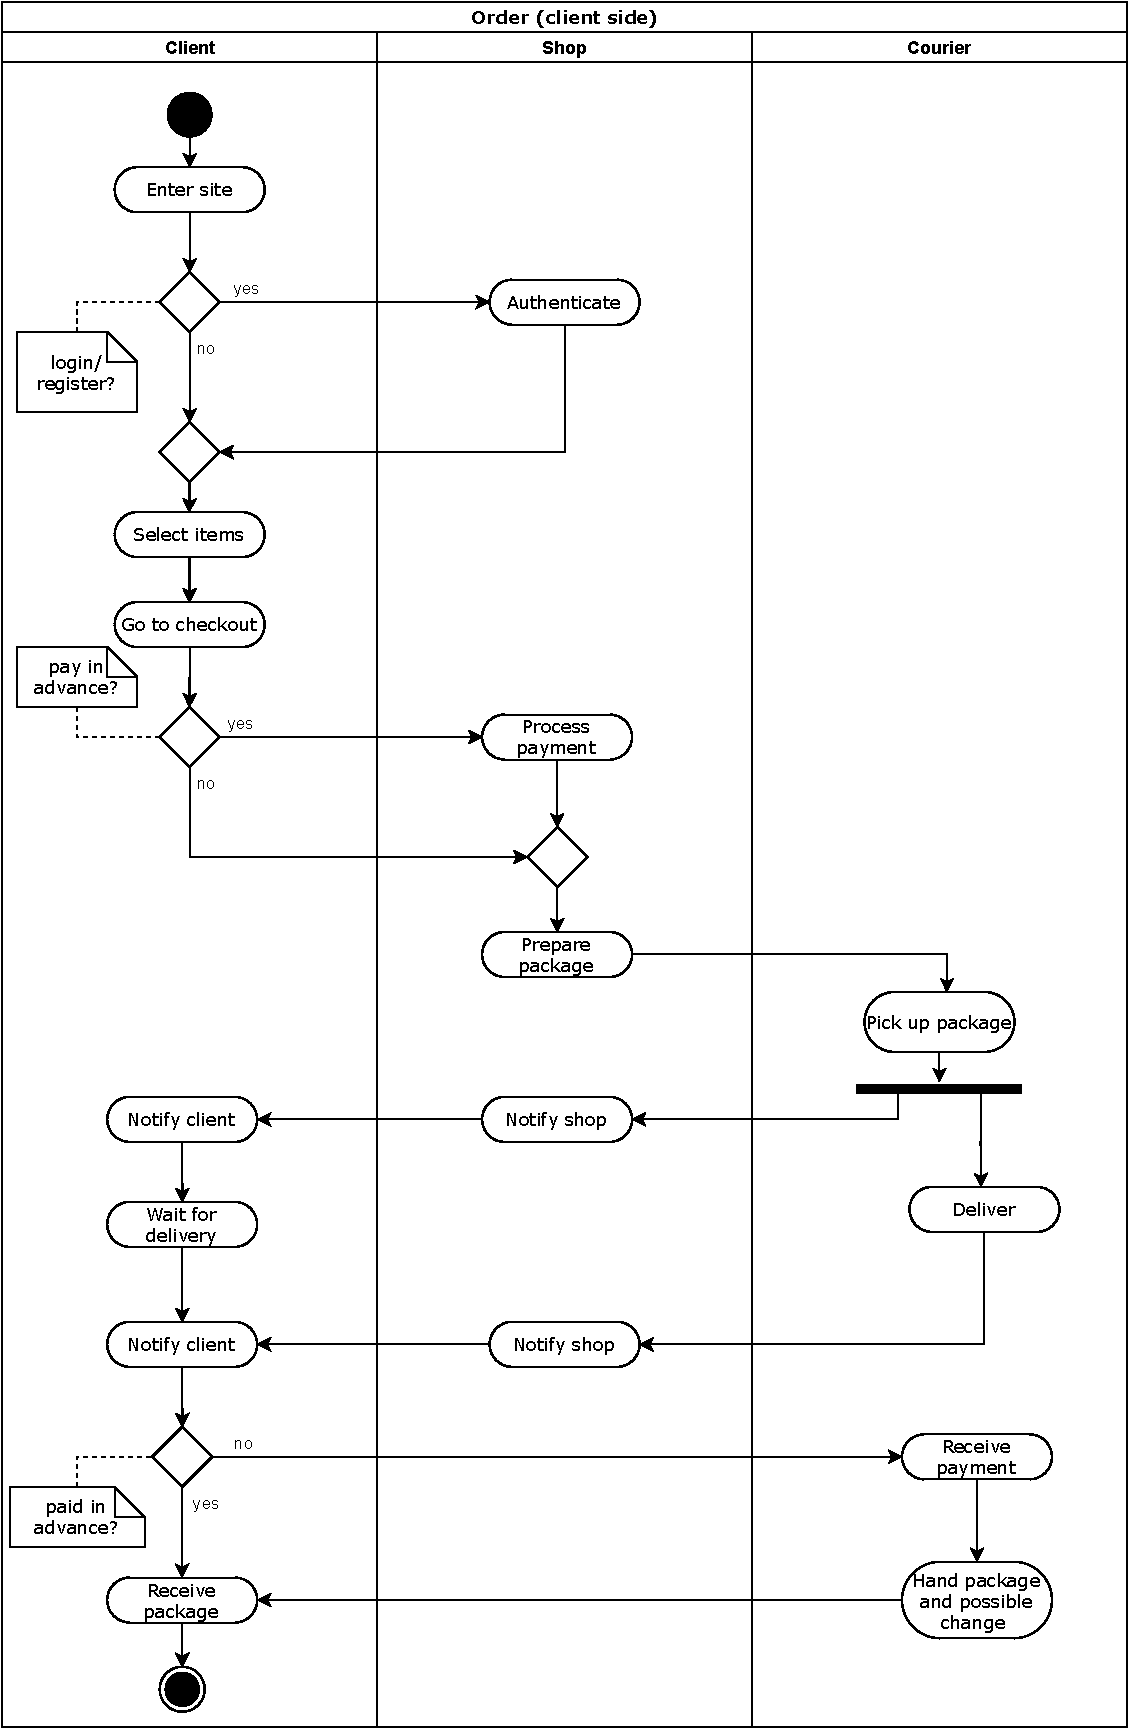
\includegraphics[width=0.75\textwidth]
{diagrams/activity-diagrams/Client-order.pdf}}
\vspace{5mm}


First action taken by a client in process of making an order is entering a website and registering (or logging if registered). After typing credentials then comes veryfing from a shop side. After successful logging client choose products he wants to order. When the list of products is completed client need to submit his choices and then choose method of payment. He can pay in advance or pay exactly to the courier. In the case of the first the payment is processed by the shop.
Then after this the package is prepared by the shop and after this is taken by courier. Courier pick up the package and sends notification to shop and client before and after the delivery. After getting package, if it paymant was not in advance client should pay for it to courier and after it the process is done.

\subsubsection{Delivery by a courier}
\vspace{5mm}
\makebox[\textwidth]{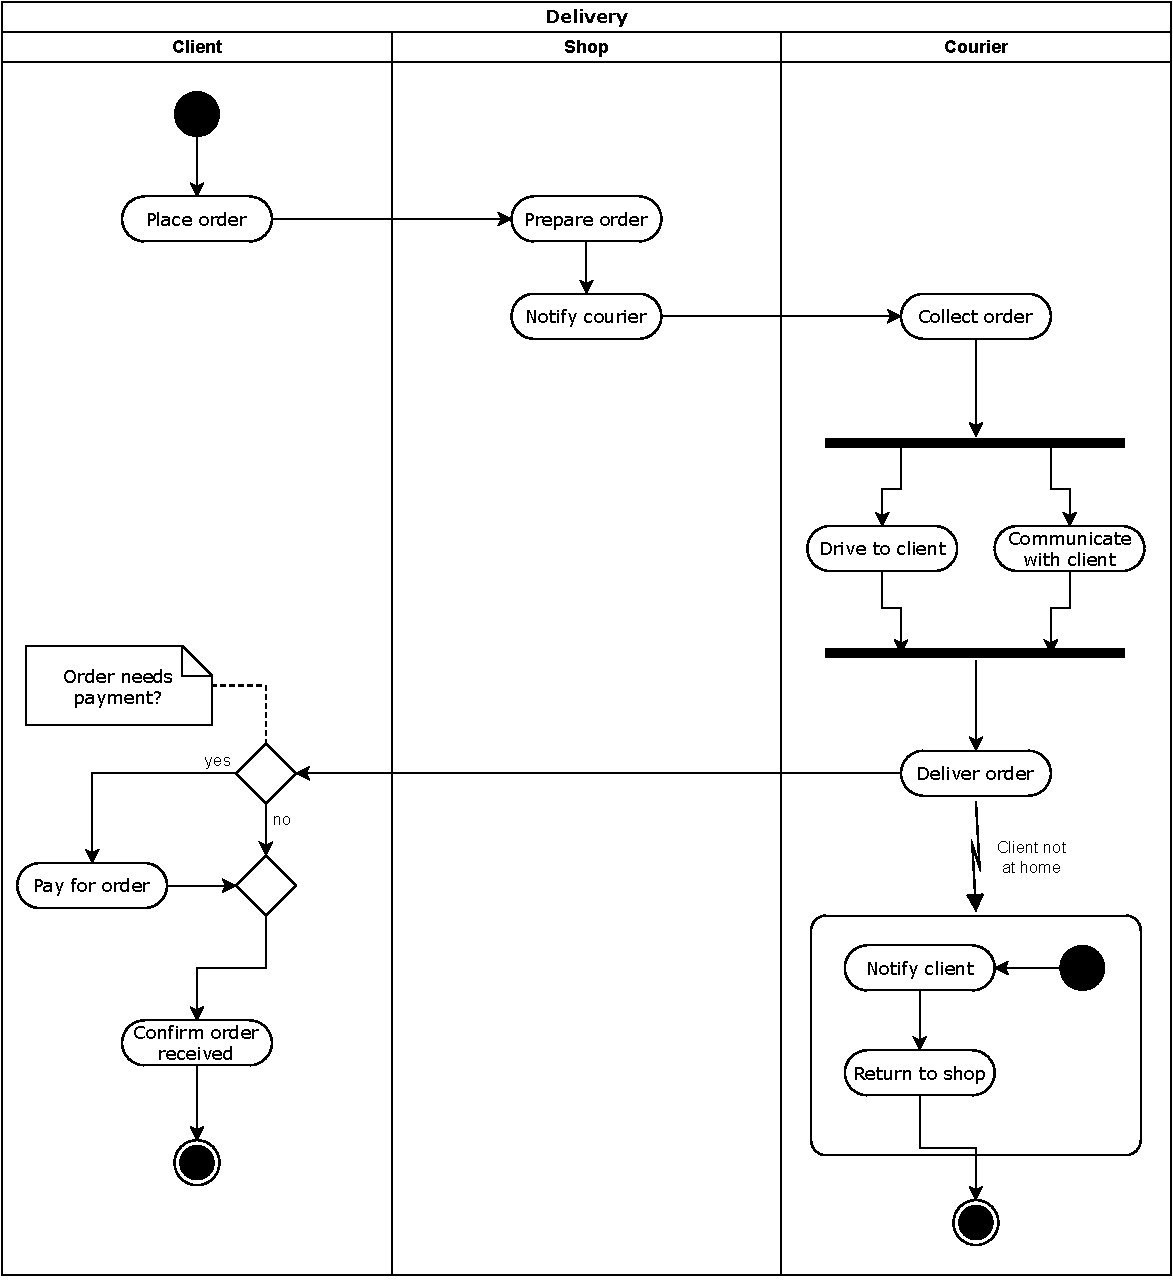
\includegraphics[width=0.75\textwidth]
{diagrams/activity-diagrams/courier-delivery.pdf}}
\vspace{5mm}


The action of delivering a product starts when a client place an order by paying for the products he has chosen before. Then it is shop job to prepare the order and as soon as they do it they have to mark it as completed and notify the courier. Courier gets notification about the order and comes for it to collect it. Then he is on his way to client and he can communicate with him to tell about his arrival or establish details with an address. When courier delivers product it is for client side to pay for it if he has not paid for it before. After that client confirms receiving products. There may happen situation that the client is not at home, in that situation courier tries to communicate with client and if there is no option to deliver it courier comes with an order back to the shop.

\subsubsection{Complaint}
\vspace{5mm}
\makebox[\textwidth]{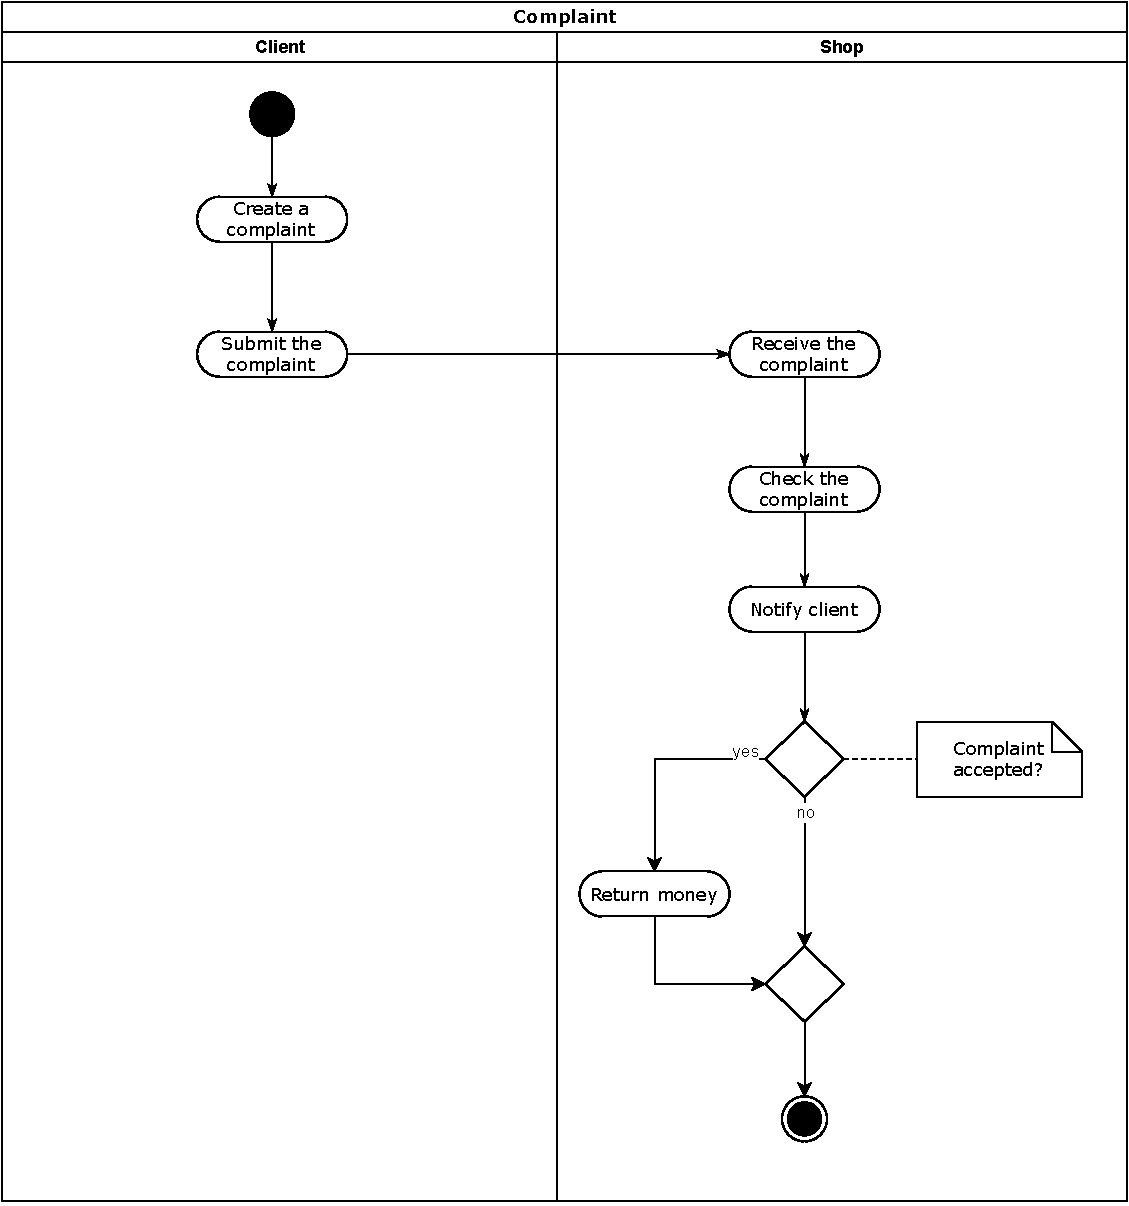
\includegraphics[width=0.75\textwidth]
{diagrams/activity-diagrams/Complaint.pdf}}
\vspace{5mm}


To start making a complaint client after receiving products must click adequate button and then select products which he does not enjoy. After submitting a complaint by the client, the shop receives it and then starts to check if it is right justified. After checking shop sends notification to client whether it was accepted or not. If yes, then money should be returned to a client.


\subsubsection{Shop preparing an order}
\vspace{5mm}
\makebox[\textwidth]{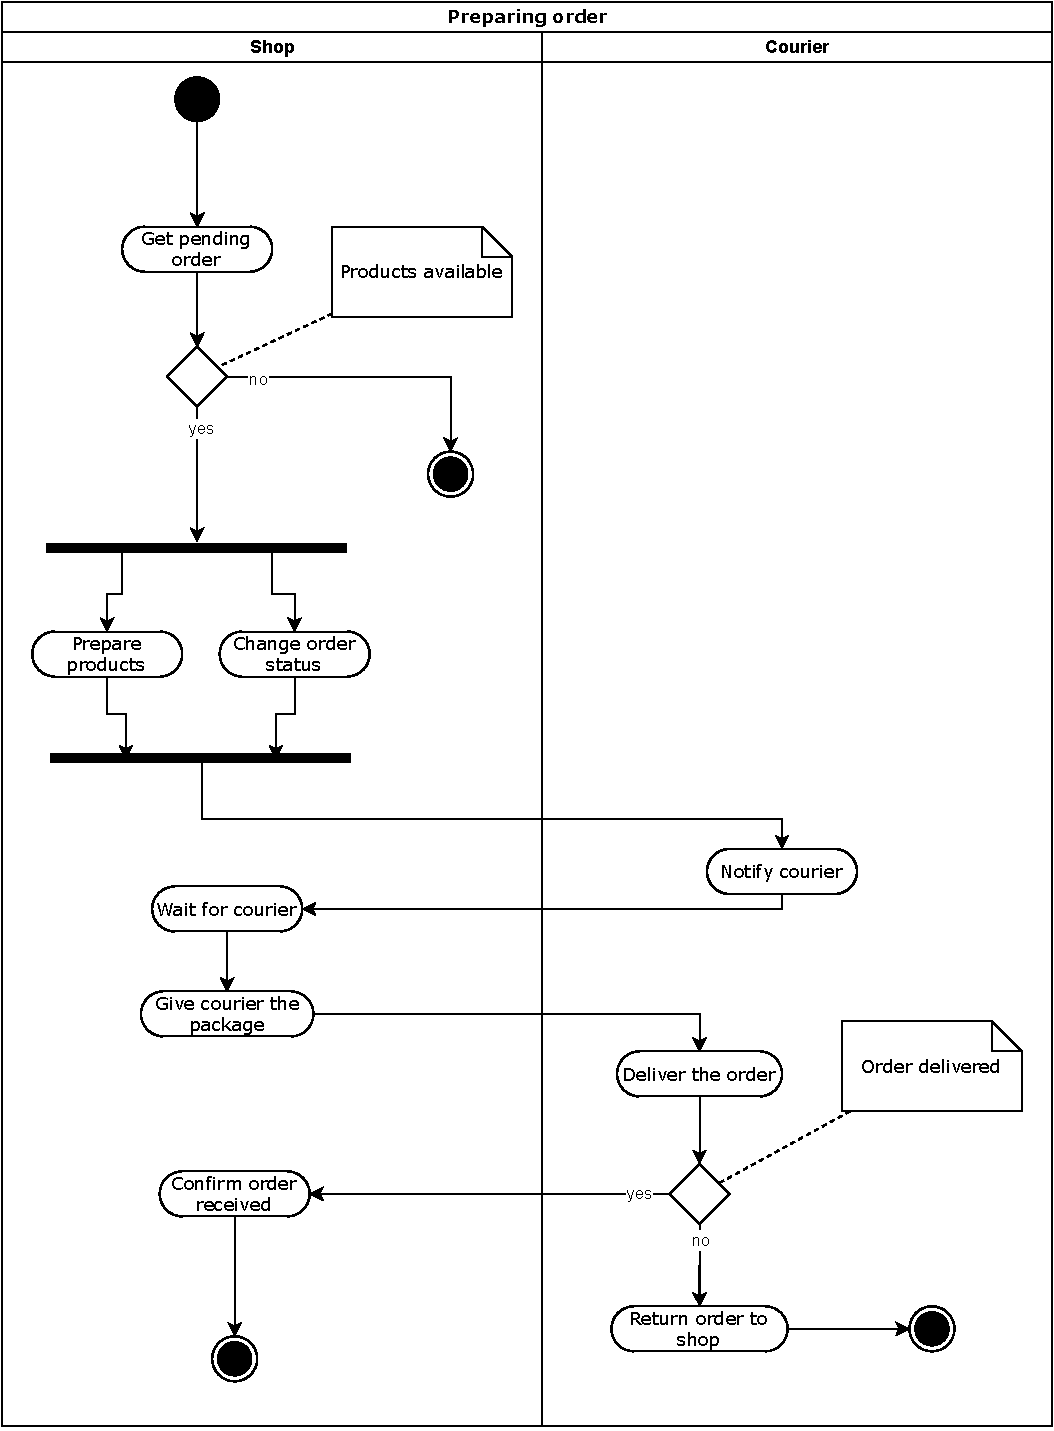
\includegraphics[width=0.75\textwidth]
{diagrams/activity-diagrams/Shop-order.pdf}}
\vspace{5mm}


To complete an order at first shop worker needs to choose order from pending orders. Then he choose from available products and pack it changing it status. After the package is completed the notification to courier is send that he can come to collect it. Courier delivers the package and in case of success there comes a confirmation of receiving an order. In other case the order is returned to shop.
\subsubsection{Shop worker}
\vspace{5mm}
\makebox[\textwidth]{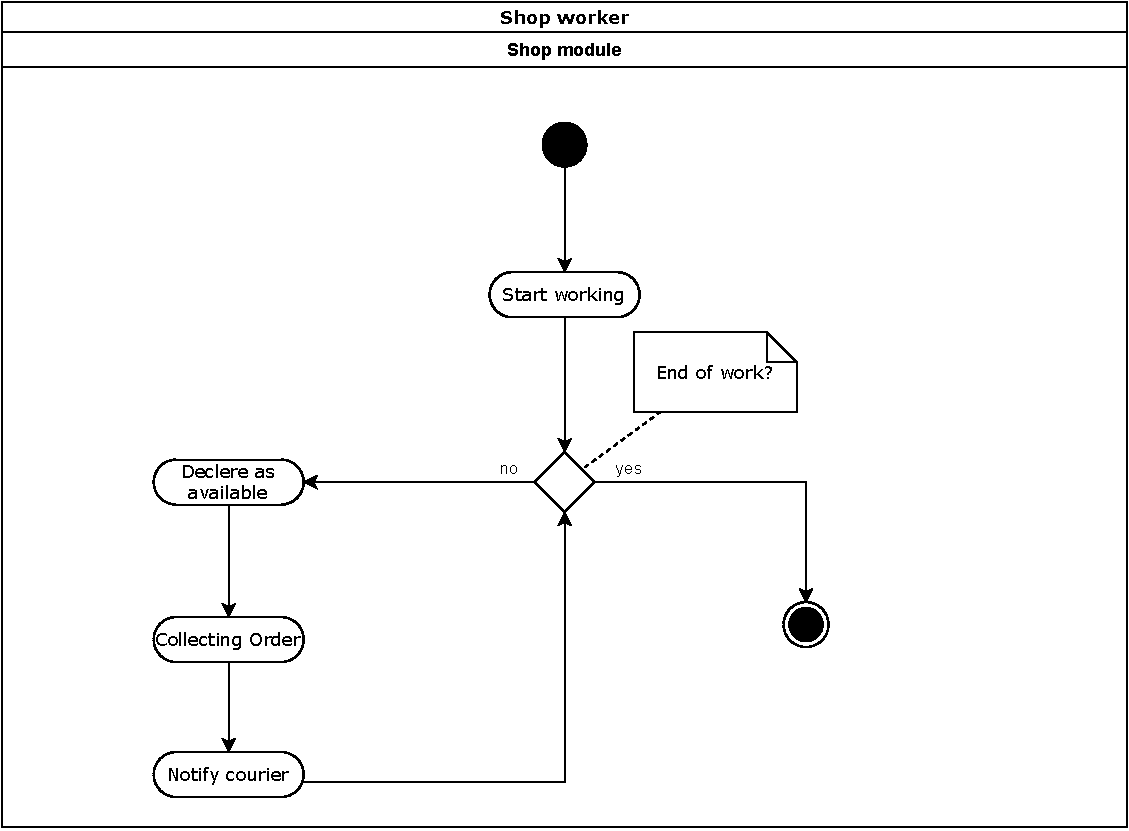
\includegraphics[width=0.75\textwidth]
{diagrams/activity-diagrams/shopworker.pdf}}
\vspace{5mm}


Shop worker is logging to the system to start work. During his shift he declares as available and when he gets an order to collect he does it. After that action he notifies the courier. If it is time to end his shift he logs out, if not he declares as available.

\end{document}